\begin{figure}[!h]
\centering
\resizebox{\columnwidth}{!}{


\tikzset{every picture/.style={line width=0.75pt}} %set default line width to 0.75pt        

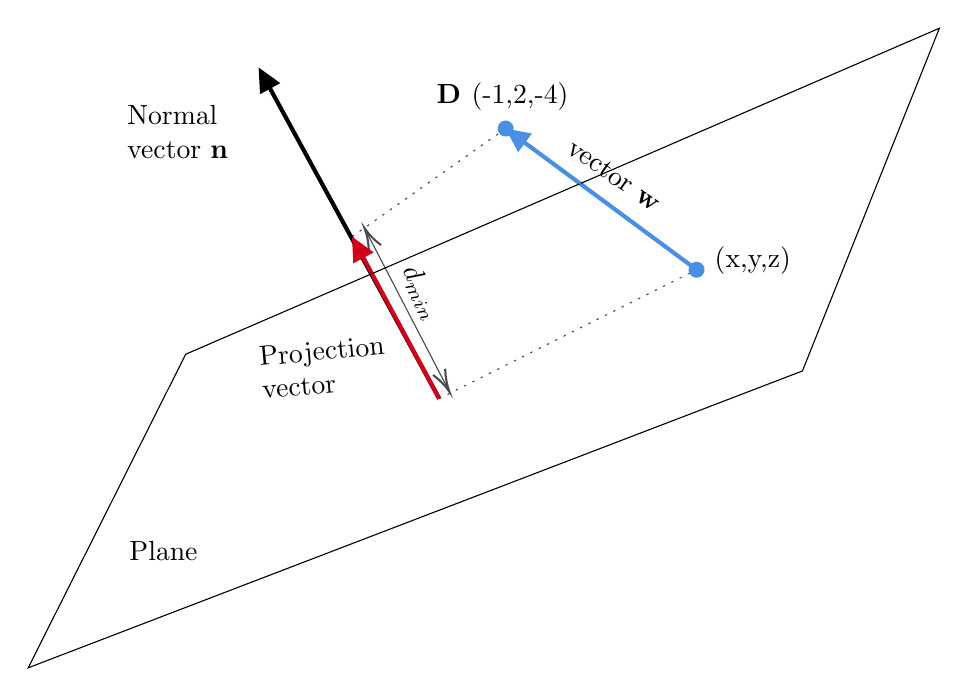
\begin{tikzpicture}[x=0.75pt,y=0.75pt,yscale=-1,xscale=1]
%uncomment if require: \path (0,324); %set diagram left start at 0, and has height of 324

%Straight Lines [id:da012474511036709712] 
\draw [color={rgb, 255:red, 74; green, 74; blue, 74 }  ,draw opacity=1 ] [dash pattern={on 0.84pt off 2.51pt}]  (165.51,108.36) -- (239.51,56.27) ;
%Straight Lines [id:da164610693713777] 
\draw [color={rgb, 255:red, 74; green, 74; blue, 74 }  ,draw opacity=1 ] [dash pattern={on 0.84pt off 2.51pt}]  (207.51,186.36) -- (331.51,124.27) ;
%Straight Lines [id:da0009900971082483778] 
\draw [color={rgb, 255:red, 74; green, 74; blue, 74 }  ,draw opacity=1 ]   (211.58,181.43) -- (172.42,105.98) ;
\draw [shift={(171.5,104.2)}, rotate = 422.57] [color={rgb, 255:red, 74; green, 74; blue, 74 }  ,draw opacity=1 ][line width=0.75]    (10.93,-3.29) .. controls (6.95,-1.4) and (3.31,-0.3) .. (0,0) .. controls (3.31,0.3) and (6.95,1.4) .. (10.93,3.29)   ;
\draw [shift={(212.5,183.2)}, rotate = 242.57] [color={rgb, 255:red, 74; green, 74; blue, 74 }  ,draw opacity=1 ][line width=0.75]    (10.93,-3.29) .. controls (6.95,-1.4) and (3.31,-0.3) .. (0,0) .. controls (3.31,0.3) and (6.95,1.4) .. (10.93,3.29)   ;
%Straight Lines [id:da6317108471264852] 
\draw [line width=1.5]    (207.51,186.36) -- (122.42,30.38) ;
\draw [shift={(120.51,26.87)}, rotate = 421.39] [fill={rgb, 255:red, 0; green, 0; blue, 0 }  ][line width=0.08]  [draw opacity=0] (11.61,-5.58) -- (0,0) -- (11.61,5.58) -- cycle    ;
%Straight Lines [id:da4711513779445873] 
\draw [color={rgb, 255:red, 74; green, 144; blue, 226 }  ,draw opacity=1 ][line width=1.5]    (331.51,124.27) -- (242.72,58.64) ;
\draw [shift={(239.51,56.27)}, rotate = 396.47] [fill={rgb, 255:red, 74; green, 144; blue, 226 }  ,fill opacity=1 ][line width=0.08]  [draw opacity=0] (11.61,-5.58) -- (0,0) -- (11.61,5.58) -- cycle    ;
%Straight Lines [id:da281513313013386] 
\draw [color={rgb, 255:red, 208; green, 2; blue, 27 }  ,draw opacity=1 ][line width=1.5]    (207.51,186.36) -- (167.4,111.89) ;
\draw [shift={(165.51,108.36)}, rotate = 421.7] [fill={rgb, 255:red, 208; green, 2; blue, 27 }  ,fill opacity=1 ][line width=0.08]  [draw opacity=0] (11.61,-5.58) -- (0,0) -- (11.61,5.58) -- cycle    ;
%Shape: Polygon [id:ds23253650680866844] 
\draw   (85.38,164.99) -- (448.5,7.93) -- (382.5,173.07) -- (9.5,316.07) -- (9.5,316.07) -- cycle ;
%Straight Lines [id:da02842289374539675] 
\draw [color={rgb, 255:red, 74; green, 144; blue, 226 }  ,draw opacity=1 ]   (239.51,56.27) -- (331.51,124.27) ;
\draw [shift={(331.51,124.27)}, rotate = 36.47] [color={rgb, 255:red, 74; green, 144; blue, 226 }  ,draw opacity=1 ][fill={rgb, 255:red, 74; green, 144; blue, 226 }  ,fill opacity=1 ][line width=0.75]      (0, 0) circle [x radius= 3.35, y radius= 3.35]   ;
\draw [shift={(239.51,56.27)}, rotate = 36.47] [color={rgb, 255:red, 74; green, 144; blue, 226 }  ,draw opacity=1 ][fill={rgb, 255:red, 74; green, 144; blue, 226 }  ,fill opacity=1 ][line width=0.75]      (0, 0) circle [x radius= 3.35, y radius= 3.35]   ;

% Text Node
\draw (56,44) node [anchor=north west][inner sep=0.75pt]   [align=left] {Normal \\vector \textbf{n} };
% Text Node
\draw (118.97,160.37) node [anchor=north west][inner sep=0.75pt]  [rotate=-354.79] [align=left] {Projection \\vector};
% Text Node
\draw (205,33) node [anchor=north west][inner sep=0.75pt]   [align=left] {\textbf{D }(-1,2,-4)};
% Text Node
\draw (339,112) node [anchor=north west][inner sep=0.75pt]   [align=left] {(x,y,z)};
% Text Node
\draw (272.66,59.12) node [anchor=north west][inner sep=0.75pt]  [rotate=-34.52] [align=left] {vector \textbf{w} };
% Text Node
\draw (198.69,119.24) node [anchor=north west][inner sep=0.75pt]  [rotate=-64.65] [align=left] {$d_{min}$};
% Text Node
\draw (57,254.07) node [anchor=north west][inner sep=0.75pt]   [align=left] {Plane};


\end{tikzpicture}
}
\caption{}
\label{eq:solutions/1/38/myfig}
\end{figure}
We are given that AB = AC. So
\begin{align}
  \norm{\vec{A-B}} = \norm{\vec{A-C}} \label{eq:solutions/1/38/eq1}
\end{align}
Also BA is produced to D such that AB = AD. Therefore we have
\begin{align}
  \vec{A-B} = \vec{D-A} \label{eq:solutions/1/38/eq2}
\end{align}
Taking dot product of vectors $\vec{(B-C)}$ and $\vec{(D-C)}$ we get
\begin{align*}
  &\vec{(B-C)}^T\vec{(D-C)}\\
  &= \vec{(B-A+A-C)}^T\vec{(D-A+A-C)}\\
  &= \vec{((B-A)+(A-C))}^T\vec{((D-A)+(A-C))}
\end{align*}
using \eqref{eq:solutions/1/38/eq2} we get
\begin{align*}
  &\vec{(B-C)}^T\vec{(D-C)} \\
  &= \vec{((B-A)+(A-C))}^T\vec{((D-A)+(A-C))}\\
  &= \vec{((B-A)+(A-C))}^T\vec{((A-B)+(A-C))}\\
  &= \vec{(-(A-B)+(A-C))}^T\vec{((A-B)+(A-C))}\\
  \begin{split}
    &= -\norm{\vec{A-B}}^2-\vec{(A-B)}^T\vec{(A-C)}\\
    &\qquad +\vec{(A-C)}^T\vec{(A-B)}+\norm{\vec{A-C}}^2
  \end{split}
\end{align*}
now $\vec{(A-B)}^T\vec{(A-C)}$ and $\vec{(A-C)}^T\vec{(A-B)}$ are both dot product of vectors $\vec{(A-B)}$ and $\vec{(A-C)}$,therefore
\begin{align*}
  &\vec{(B-C)}^T\vec{(D-C)}\\
  \begin{split}
    &= -\norm{\vec{A-B}}^2-\vec{(A-B)}^T\vec{(A-C)}\\
                                &\qquad +\vec{(A-C)}^T\vec{(A-B)}+\norm{\vec{A-C}}^2
  \end{split}\\
  &= -\norm{\vec{A-B}}^2+\norm{\vec{A-C}}^2
\end{align*}
using \eqref{eq:solutions/1/38/eq1} we get
\begin{align}
  \vec{(B-C)}^T\vec{(D-C)} &= -\norm{\vec{A-B}}^2+\norm{\vec{A-C}}^2 = 0
\end{align}
since $\vec{(B-C)}^T\vec{(D-C)}$ = 0,therefore BC $\perp$ CD and $\angle{BCD}$ is a right angle.
